\documentclass{TDP003mall}
\definecolor{terminalgreen}{HTML}{8AE234}
\usepackage{graphicx} 
\usepackage{wrapfig}

\newcommand{\version}{Version 1.0}
\author{Eric Jönsson, \url{erijo137@student.liu.se}\\
  Ida Bergquist, \url{idabe112@student.liu.se}}
\title{Installationsmanual}
\date{2018-09-19}
\rhead{Ida Bergquist\\
Eric Jönsson}



\begin{document}
\projectpage
\section{Revisionshistorik}
\begin{table}[!h]
\begin{tabularx}{\linewidth}{|l|X|l|}
\hline
Ver. & Revisionsbeskrivning & Datum \\\hline
1.0 & Skapade installationsmanualen & 180919 \\\hline
\end{tabularx}
\end{table}

\section{Förinstallationskrav}
Portfolion förlitar sig på följande program för att fungera korrekt:\\
\begin{enumerate}
\item Python3
\item Pip
\item Flask
\item Jinja2
\end{enumerate}
Se till att ha de senaste versionerna av programmen innandu installerar portfolion.\\
Nedan hittar du instruktioner för att installera och uppdatera programmen. Instruktionerna är skrivna för debian-baserade linuxdistrubitioner, ex. Ubuntu, Linux Mint etc\ldots
\subsection{Python}
Installera Python3 genom att skriva förjande kommando i terminalen:\\
\textbf{\textcolor{terminalgreen}{user@computer}:\~{}\$ sudo apt install python3} \\
Uppdatera python3 genom att skriva:\\
\textbf{\textcolor{terminalgreen}{user@computer}:\~{}\$ sudo apt update \&\& sudo apt upgrade python3}\\
Installera även python3-venv.\\
\textbf{\textcolor{terminalgreen}{user@computer}:\~{}\$ sudo apt install python3-venv}\\

\subsection{Pip}
Installera pip genom terminalen:\\
\textbf{\textcolor{terminalgreen}{user@computer}:\~{}\$ sudo apt install python-pip}\\

\newpage
\subsection{Flask och Jinja2}
\begin{wrapfigure}{r}{0.4\textwidth}
    \begin{center}
        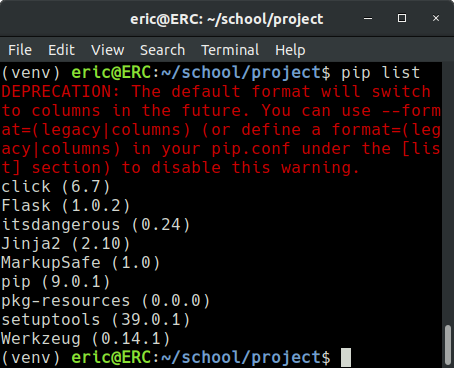
\includegraphics[width=0.40\textwidth]{./list2.png}
    \end{center}
\end{wrapfigure}
Innan Flask installeras behöver du skapa en mapp där du vill installera portfolion. Gå sedan in i den mappen och starta terminalen. Högerklicka i mappen och tryck på "Open in terminal" i menyn. Sedan behöver du ska en virtuell miljö för att portfolion inte ska gå sönder vid framtida uppdateringar. Skriv följande kommando i terminalen:\\
\textbf{\textcolor{terminalgreen}{user@computer}:\~{}\$ python3 -m venv venv}\\
Flask och Jinja2 installeras via pip. Skriv följande kommando i terminalen:\\
( venv ) \textbf{\textcolor{terminalgreen}{user@computer}:\~{}\$ pip install Flask}\\
När Flask installeras ingår flera paket, bl.a. Jinja2.
För att kontrollera att du nu har både Flask och Jinja2 kan du skriva följande i terminalen:\\
( venv ) \textbf{\textcolor{terminalgreen}{user@computer}:\~{}\$ pip list}\\
Kontrollera att både Flask och Jinja2 finns med i listan.
\section{Installation för Linux}
Öppna mappen du vill installera portfolion i. Högerklicka i mappen och tryck på "Open in terminal". Skriv sedan följande kommando i terminalen:\\
( venv ) \textbf{\textcolor{terminalgreen}{user@computer}:\~{}\$ git clone git@gitlab.ida.liu.se:erijo137/Portfolioprogram}\\
Du ska nu kunna installera portfolion genom att skriva följande i terminalen:\\
( venv ) \textbf{\textcolor{terminalgreen}{user@computer}:\~{}\$ pip install -e .}\\


\end{document}
